\documentclass[a4paper,UTF8]{article}
\usepackage{ctex}
\usepackage[margin=1.25in]{geometry}
\usepackage{color}
\usepackage{graphicx}
\usepackage{amssymb}
\usepackage{amsmath}
\usepackage{amsthm}
%\usepackage[thmmarks, amsmath, thref]{ntheorem}
\theoremstyle{definition}
\newtheorem*{solution}{Solution}
\newtheorem*{prove}{Proof}
\usepackage{multirow}
\usepackage{url}
% 设置linkcolor为黑色,urlcolor为蓝色
\usepackage[colorlinks,linkcolor=black,urlcolor=blue]{hyperref}
\usepackage{enumerate}
\renewcommand\refname{参考文献}


%--

%--
\begin{document}
\title{\textbf{《计算机图形学》课程大作业实验报告}}
\author{XXX,XXX,\href{mailto:211240045@smail.nju.edu.cn}{211240045@smail.nju.edu.cn}}
\maketitle
\tableofcontents 
\newpage
\section{综述}

\subsection{2024年3月}

$\bullet$ 完成绘制直线(DDA算法)

$\bullet$ 完成绘制直线(Bresenham算法)

$\bullet$ 实现gui重置画布

$\bullet$ 实现gui保存画布

\subsection{2024年4月}

$\bullet$ 完成绘制多边形(DDA算法)

$\bullet$ 完成绘制多边形(Bresenham算法)

$\bullet$ 完成绘制椭圆(中点圆生成算法)

$\bullet$ 完成绘制曲线(Bezier算法)

$\bullet$ 完成绘制曲线(B-spline算法)

$\bullet$ 完成图元平移

$\bullet$ 完成图元旋转

$\bullet$ 完成图元缩放

$\bullet$ 实现gui设置画笔颜色

\subsection{2024年5月}

$\bullet$ 完成图元(线段)裁减(Cohen-Sutherland算法)

$\bullet$ 完成图元(线段)裁减(Liang-Barsky算法)

$\bullet$ 完成命令行界面(CLI)程序

\subsection{2024年6月}

$\bullet$ 完成系统报告

$\bullet$ 完成系统使用说明书

$\bullet$ 录制系统演示视频

\section{图元绘制算法介绍}

\subsection{绘制直线}

\subsubsection{DDA算法}

\textbf{算法原理:}DDA算法的核心思想是通过计算斜率来确定每个像素点的位置,从而形成一条连续的直线。通过坐标轴上以单位间隔取样($\Delta x = 1$或$\Delta y = 1$),因为取单位间隔,所以显见对应的$\Delta y = k, -k$或$\Delta x = \frac{1}{k},-\frac{1}{k}$(记直线为$y=kx+b$)。当起始点在左侧取值,起始点在右侧取负值。

\textbf{算法改进:}可利用直线构成的连贯性,通过将增量$k$和$\frac{1}{k}$分离成整数和小数部分从而使所有的计算都简化为整数操作来改善DDA算法的性能。

\subsubsection{Bresenham算法}

\textbf{算法原理:}通过坐标轴上以单位间隔取样($\Delta x = 1$或$\Delta y = 1$),不失一般性取$0\leq k<1$。假设$(x_k,y_k)$为已经确定的像素坐标,那么下一个像素坐标为$(x_{k}+1,y_k)$或$(x_k+1,y_k+1)$,确定$y$轴坐标选择哪一个的依据是判断直线和$x=x_k+1$的交点的$y$轴坐标与$y_k+1,y_k$哪个的绝对差值更小。若与$y_k$绝对差值更小,则下一个点选择$(x_k+1,y_k)$;若与$y_k+1$绝对差值更小,则下一个点选择$(x_k+1,y_k+1)$。

\textbf{算法改进:}为进一步提高算法效率,可以利用线段本身的对称性。用Bresenham算法产生起点一侧的半条线段,至于终点一侧的半条线段,可以看作以终点为起点线段的生成。起点一侧的线段像素坐标在$x$或$y$方向每前进一个坐标单位,终点一侧的线段像素坐标就在$x$或$y$方向后退一个坐标单位。

\subsubsection{方法对比}

DDA算法的优点在于适用面广,实现简单。但是它存在一个问题,在计算斜率时会产生精度损失,从而使得绘制出来的直线可能出现明显的锯齿状。因此,在对线条的精度有较高要求的情况下,可以采用Bresenham算法。

Bresenham算法通过整数计算来绘制线条,避免了DDA算法中的精度损失问题。因此,Bresenham算法具有更高的绘制速度和较好的像素级别的控制,可以在需要绘制直线的情况下带来更好的性能和画质。

总的来说,Bresenham算法比DDA算法绘制直线更准确高效。

\subsection{绘制多边形}

绘制多边形的方法基于绘制直线的算法,对于多边形的每条边,获得其两端点后利用直线绘制算法进行绘制即可。

\subsection{绘制椭圆}

\subsubsection{中心椭圆生成算法}

\textbf{算法原理:}算法类似于Bresenham算法,不失一般性,考虑中心在原点处的椭圆,研究第一象限。将第一象限中椭圆切线绝对值等于1所对应的切点记作临界点$P$,$P$上方的点$\frac{dy}{dx}<1$,$P$下方的点$\frac{dy}{dx}>1$,由此可利用Bresenham算法解决选点问题。根据参数方程定义椭圆函数为:
$$f_{ellipse}(x,y)=b^2x^2+a^2y^2-a^2b^2$$
在$P$上方的点,取$x$方向单位步长,再通过决策函数判断真实值与两候选像素之间哪个位置更近,更新对应的$y$值;在$P$下方的点,取$y$方向单位步长,再通过决策函数判断真实值与两候选像素之间哪个位置更近,更新对应的$x$值。又因为椭圆四个象限是互相对称的,可以通过改变对应的符号补全其余象限,最后结合中心点的实际坐标即可计算出待绘制椭圆的点坐标。

\subsection{绘制曲线}

\subsubsection{Bezier算法}

\textbf{算法原理:}Bezier算法是由多边形控制,逼近多边形的一种曲线。其做法是通过Bezier基函数来得到绘制点的坐标。Bezier基函数的原型比较复杂,但我了解到Bezier曲线基函数已被证明可简化为伯恩斯坦基函数,其形式为:

$$C_n^it^i(1-t)^i$$

有了基函数,自然可以用参数$t$,取某一个步长,来近似绘制曲线。下面以4个点控制的曲线为例,介绍算法执行步骤,其中算法接受参数中的顶点序列应当是有序的:

\noindent 1. 对两两相邻点求中点,得到三个中点

\noindent 2. 对得到的三个中点再次求中点,得到两个中点

\noindent 3. 对得到的两个中点再次求中点,得到一个中点

\noindent 4. 将得到的最接近曲线的7个点根据最后计算得到的中点对半分为每方4个,即:$P_0^0,P_0^1,P_0^2,P_0^3$和$P_0^3,P_1^2,P_2^1,P_3^0$ 

\noindent 5. 分别对这两组4个点调用上述算法,递归直到误差在可接受范围内

\subsubsection{B-spline算法}

\textbf{算法原理:}由于Bezier曲线调整的时候有“牵一发而动全身”的缺点,因此引入B-spline(B样条)曲线。B样条曲线同样拥有自己的基函数,这些基函数在定义曲线时起到关键作用。与贝塞尔曲线不同,B样条曲线的基函数具有局部影响的特点,即当调整曲线上的一个控制点时,只有曲线的一小部分会受到影响,而不是整个曲线。这种局部影响的特性是通过基函数的支撑区间(support interval)概念来实现的。

支撑区间指的是基函数值非零的区间。对于三次贝塞尔曲线,其四个基函数的支撑区间都是整个定义域[0,1],这意味着任何一个控制点的调整都会对曲线的整体形状产生影响。而B样条曲线的基函数则具有更短的支撑区间,这允许控制点的局部调整,从而提高了曲线的可控性和灵活性。

B样条曲线的基函数产生使用递推形式,即de-BoorCox递推定义:

\begin{center}
	$
	\begin{cases}  
		N_{i,1}(u)=\begin{cases}
			1,	& u_i < u < u_{i+1}	\\
			0, 	& o.t.
		\end{cases} \\
		N_{i,k}(u)=\frac{u-u_i}{u_{i+k-1}-u_i}N_{i,k-1}(u)+\frac{u_{i+k}-u}{u_{i+k}-u_{i-1}}N_{i+1,k-1}(u)
	\end{cases} 
	$	\\
	\textbf{规定$\frac{0}{0}=0$}
\end{center}

其中$k$是阶数,$u$是参数。

均匀B样条基函数是指当节点向量按照等间隔排列,即节点向量为$0,1,2,...,n+k$时,其中$n$是控制点的数量,而$k$是基函数的阶。这种均匀分布的节点向量保证了B样条曲线的基函数在整个定义域内具有相同的支撑区间,从而使得曲线在各个部分的局部控制能力相同。相对地,准均匀B样条基函数则是指节点向量的前$k$个和后$k$个元素相等,而中间的元素则均匀分布。这种分布方式允许基函数在曲线的某些部分具有更大的控制力,而在其他部分则相对较小。

针对实验要求使用均匀B样条函数的情况,为了优化性能,我们可以选择一个简化的节点向量,即仅包含从$0$到$n+k$的连续整数序列。在实际的编程实现中,代码可以按照如下形式编写:

\begin{center}
	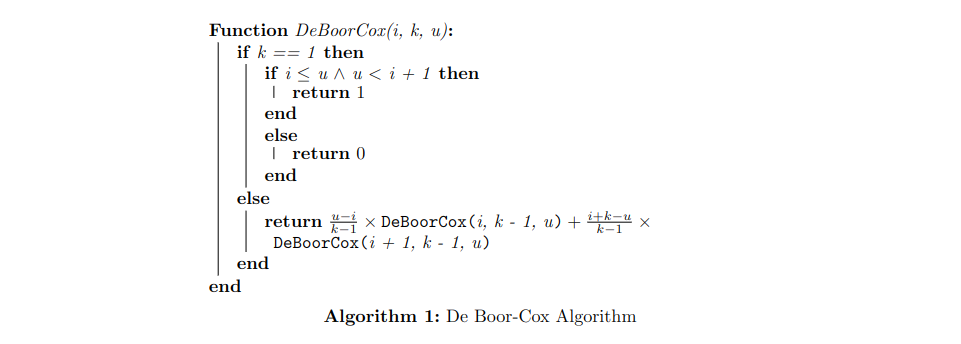
\includegraphics[width=6in]{报告/algorithm1.png}
\end{center}

\subsubsection{方法对比}

\begin{itemize}
	\item \textbf{控制点影响范围}:
	\begin{itemize}
		\item 贝塞尔曲线:任一控制点的移动都会影响整条曲线。
		\item B样条曲线:控制点主要影响曲线的局部区域。
	\end{itemize}
	
	\item \textbf{曲线表达式}:
	\begin{itemize}
		\item 贝塞尔曲线:$\vec{P}(t) = \sum_{i=0}^{n-1} \vec{p}_i B_{i,n}(t)$.
		\item B样条曲线:$\vec{P}(t) = \sum_{i=0}^{n-1} \vec{p}_i B_{i,d}(t)$.
	\end{itemize}
	
	\item \textbf{参数 $t$ 的取值范围}:
	\begin{itemize}
		\item 贝塞尔曲线:$t$ 的取值通常为 $[0, 1]$.
		\item B样条曲线:$t$ 的取值范围更广,由节点向量定义。
	\end{itemize}
	
	\item \textbf{局部性与连续性}:
	\begin{itemize}
		\item 贝塞尔曲线:不具备局部性,但连续性容易满足。
		\item B样条曲线:具有局部性,可以构造出高阶连续的曲线。
	\end{itemize}
	
	\item \textbf{几何属性}:
	\begin{itemize}
		\item 贝塞尔曲线:几何属性简单,易于理解。
		\item B样条曲线:具有变差缩减性、凸包性、仿射不变性等复杂几何属性。
	\end{itemize}
	
	\item \textbf{应用场景}:
	\begin{itemize}
		\item 贝塞尔曲线:适用于简单图形设计,如字体设计。
		\item B样条曲线:适用于复杂曲面建模,如CAD/CAM系统。
	\end{itemize}
	
	\item \textbf{计算复杂度}:
	\begin{itemize}
		\item 贝塞尔曲线:计算简单,适合实时应用。
		\item B样条曲线:计算复杂,提供更高的设计灵活性。
	\end{itemize}
	
	\item \textbf{节点向量 (Knot Vector)}:
	\begin{itemize}
		\item 贝塞尔曲线:不使用节点向量。
		\item B样条曲线:使用节点向量来定义曲线的局部控制范围。
	\end{itemize}
\end{itemize}

\section{图元变换算法介绍}

\subsection{图元平移}

\subsubsection{算法原理}

不妨设$dx$为水平方向平移量,$dy$为垂直方向平移量。

$x,y$为原始坐标,$x',y'$为平移后坐标,则:

\begin{center}
$
	\begin{cases}  
		x'=x+dx\\
		y'=y+dy    
	\end{cases} 
$
\end{center}

\subsubsection{算法实现}

需要实现或改动的函数有:

$\bullet$ start\_translate函数

$\bullet$ mousePressEvent函数

$\bullet$ mouseMoveEvent函数

$\bullet$ mouseReleaseEvent函数

$\bullet$ MainWindow类中连接槽函数,实现translate\_action函数

在start\_translate函数将当前系统状态调整为translate;在mousePressEvent函数中确定平移对象并记录初始位置;在mouseMoveEvent函数中随着鼠标指针移动,调用alg.translate函数更新平移对象的点集坐标,然后刷新界面。由此,即可实现平移功能。

\subsection{图元旋转}

\subsubsection{算法原理}

不妨设$x_r,y_r$为旋转中心点坐标,$\theta$为旋转角度。

$x,y$为原始坐标,$x',y'$为旋转后坐标,则:

\begin{center}
	$
	\begin{cases}  
		x'=x_r+(x-x_r)\cos\theta - (y-y_r)\sin\theta \\
		y'=y_r+(x-x_r)\sin\theta + (y-y_r)\cos\theta 
	\end{cases} 
	$
\end{center}

\subsubsection{算法实现}

需要实现或改动的函数有:

$\bullet$ start\_rotate函数

$\bullet$ mousePressEvent函数

$\bullet$ mouseMoveEvent函数

$\bullet$ mouseReleaseEvent函数

$\bullet$ MainWindow类中连接槽函数,实现rotate\_action函数

在start\_rotate函数将当前系统状态调整为rotate;在mousePressEvent函数中第一次点击确定旋转中心,第二次点击确定旋转起始位置;在mouseMoveEvent函数中随着鼠标指针移动,计算顺时针旋转角度参数r,调用alg.rotate函数更新旋转对象的点集坐标,然后刷新界面。由此,即可实现旋转功能。

\subsection{图元缩放}

\subsubsection{算法原理}

不妨设$x_f,y_f$为缩放中心点坐标,$s$为缩放倍数。

$x,y$为原始坐标,$x',y'$为缩放后坐标,则:

\begin{center}
	$
	\begin{cases}  
		x'=x\cdot s + x_f\cdot (1-s) \\
		y'=y\cdot s + y_f\cdot (1-s) 
	\end{cases} 
	$
\end{center}

\subsubsection{算法实现}

需要实现或改动的函数有:

$\bullet$ start\_scale函数

$\bullet$ mousePressEvent函数

$\bullet$ mouseMoveEvent函数

$\bullet$ mouseReleaseEvent函数

$\bullet$ MainWindow类中连接槽函数,实现scale\_action函数

在start\_scale函数将当前系统状态调整为scale;在mousePressEvent函数中第一次点击确定缩放中心,第二次点击确定缩放起始位置;在mouseMoveEvent函数中随着鼠标指针移动,计算缩放倍率参数s,调用alg.scale函数更新缩放对象的点集坐标,然后刷新界面。由此,即可实现缩放功能。

\subsection{图元裁剪}

\subsubsection{算法原理——Cohen-Sutherland算法}

编码算法将整个画布分成九个区域,如下图所示:

\begin{center}
	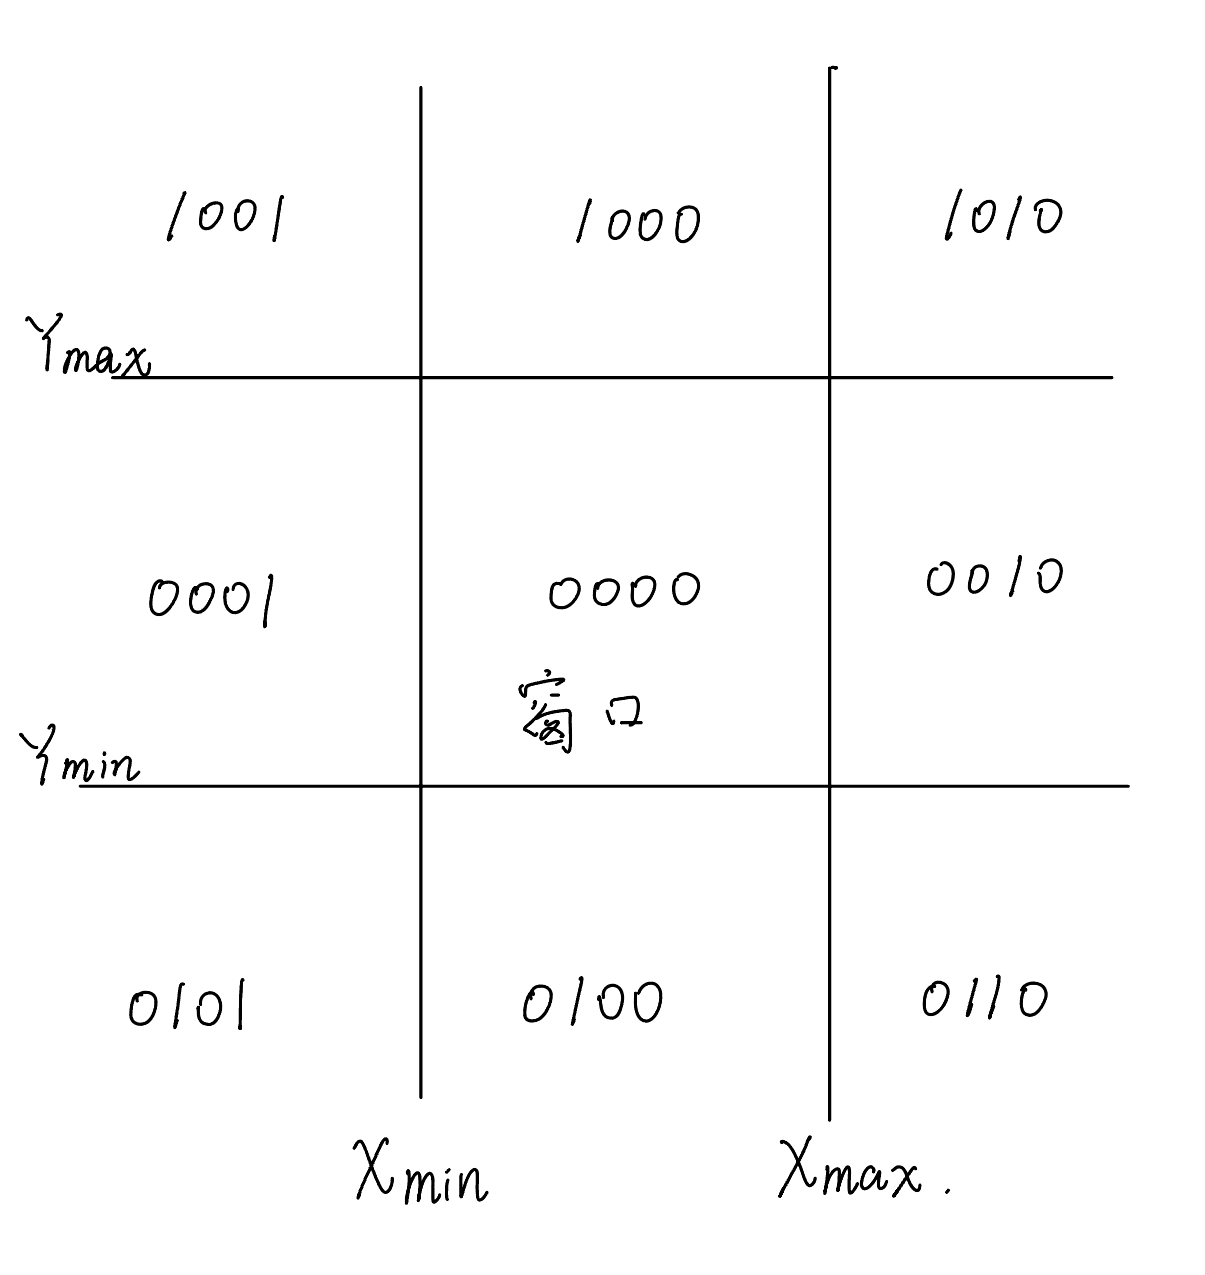
\includegraphics[width=4in]{报告/1.png}
\end{center}

根据线段端点所在位置,给每个端点一个四位二进制码(称为区域码)。四位区域码的4位从左到右以此表示为上、下、右、左。区域码的任何位赋值为1代表端点落在相应的区域中,否则为0。

据区域编码规则可知,在确定区域码每位的值时,可通过比较端点坐标值$(x,y)$和裁剪边界来确定区域码各位的值:

如果$x<x_{min}$,表示该点在裁剪窗口左边界的左方,则第1位置1,否则置0;

如果$x>x_{max}$,表示该点在裁剪窗口右边界的右方,则第2位置1,否则置0;

如果$y<y_{min}$,表示该点在裁剪窗口下边界的下方,则第3位置1,否则置0;

如果$y>y_{max}$,表示该点在裁剪窗口上边界的上方,则第4位置1,否则置0。

根据线段和裁剪窗口的关系,可分三种情况进行处理:

线段完全在裁剪窗口之内,两个端点的区域码都为0000,则该线段完全在裁剪窗口内;

线段完全在裁剪窗口之外,两个端点的区域码相与的结果不为0000,则该线段完全在裁剪窗口之外;

其他情况下,显见属于一半落在窗口内一半落在窗口外,线段将被裁剪,需要进行求交运算。首先对线段外端点(落在窗口外的点)与一条裁剪边界比较来确定需要裁剪多少线段;然后,将线段的剩下部分与其他裁剪边界对比,直到该直线完全落在窗口内或者被舍弃。实际算法实现只有在检测到区域码的某位为1时,才把线段和对应裁剪窗口进行求交运算。

\subsubsection{算法原理——Liang-Barsky算法}

Liang-Barsky算法有两个主要思想:用参数方程表示直线;将待裁剪直线看作一有方向的线。

\textbf{用参数方程表示直线}

设待裁剪线段为$P_1P_2$,其中$P_1=(x_1,y_1),P_2=(x_2,y_2)$,用参数$u$表示如下直线:

\begin{center}
	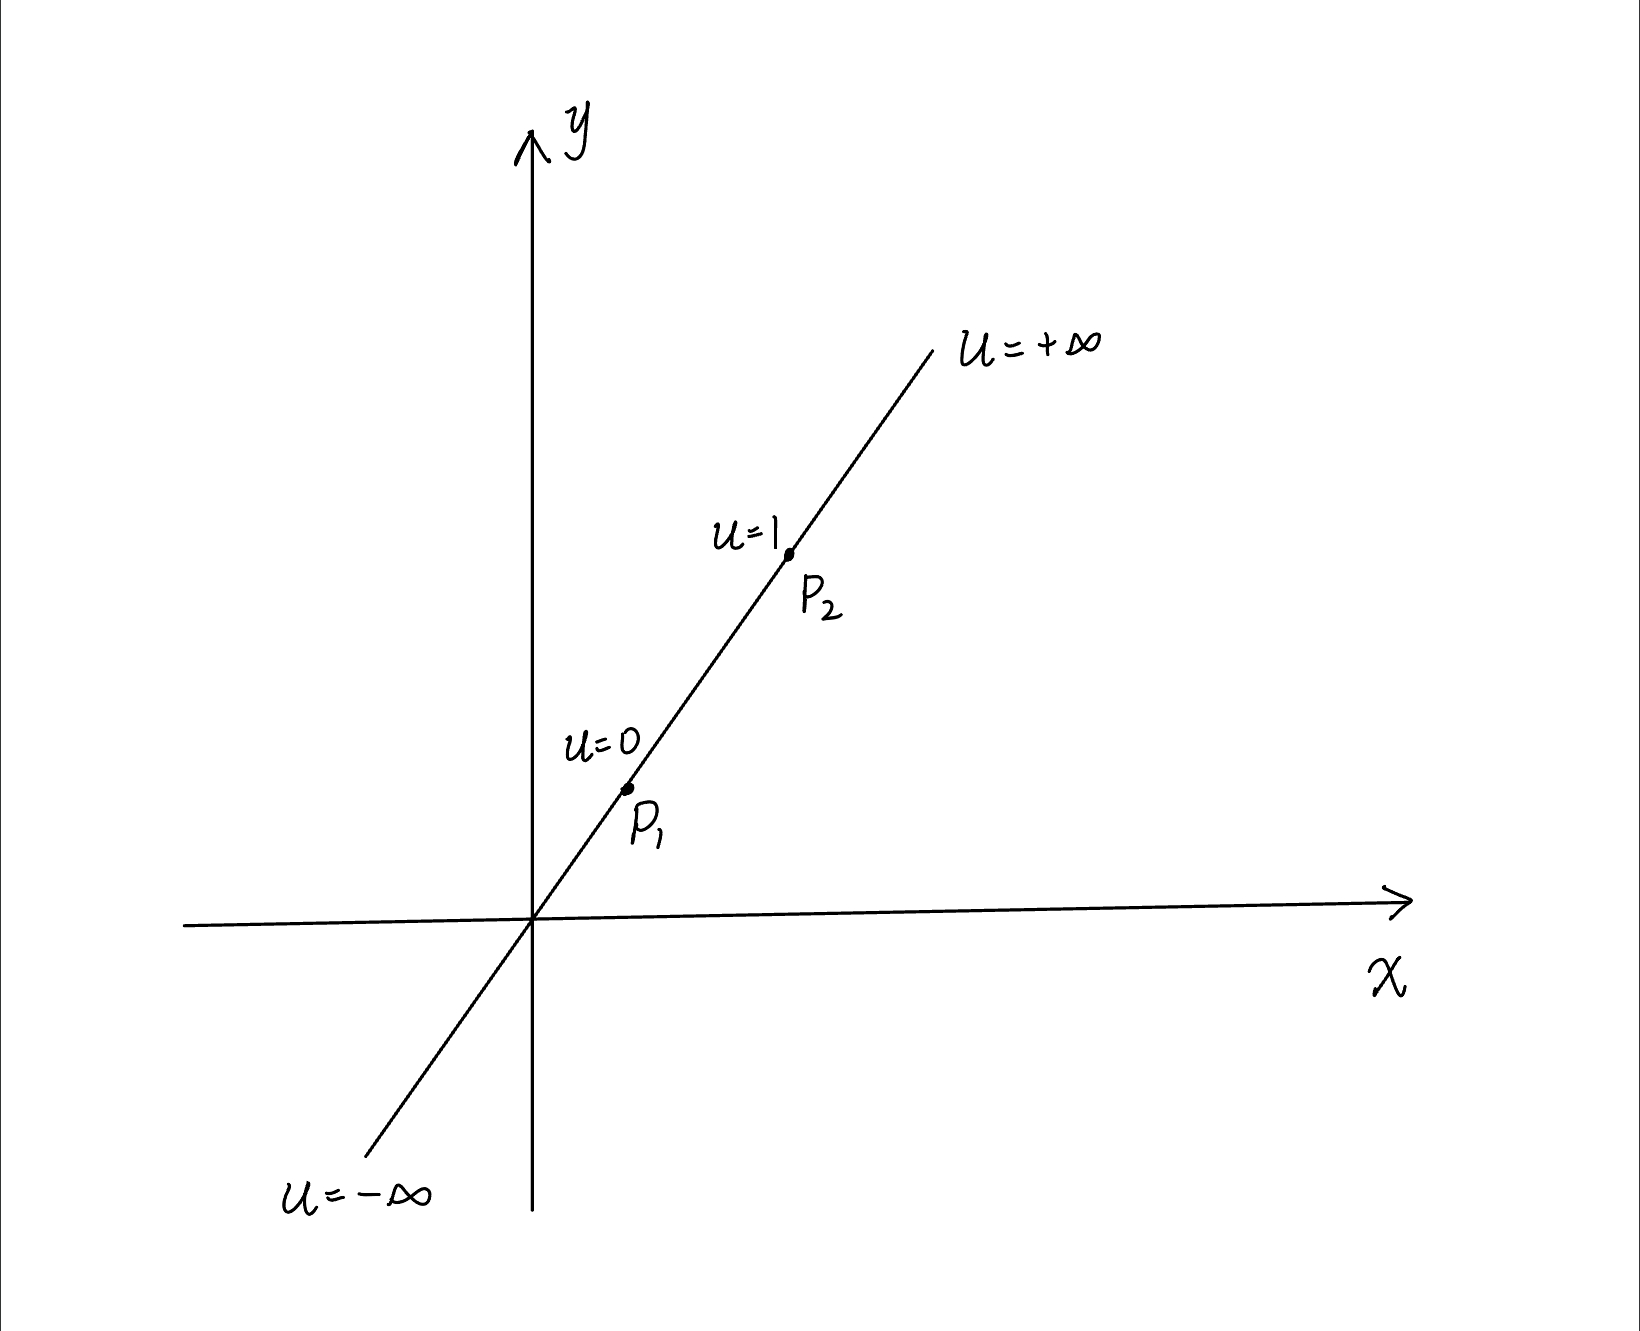
\includegraphics[width=4in]{报告/2.png}
\end{center}

\begin{center}
	$
	\begin{cases}  
		x=x_1+u(x_2-x_1) = x_1 + u\Delta x\ \ 0\leq u\leq 1 \\
		y=y_1+u(y_2-y_1) = y_1 + u\Delta y\ \ 0\leq u\leq 1 
	\end{cases} 
	$
\end{center}

当$u=0$时,$x=x_1,y=y_1$,也就是$P_1$;当$u=1$时,$x=x_2,y=y_2$,也就是$P_2$;当$u=0.5$时,为$P_1P_2$中点。

\textbf{将待裁剪直线看作一有方向的线}

根据$u$的取值,可以确定所需裁剪的线段的多少,那么$u$如何取值?

我们将裁剪窗口的四个边分为入边和出边两类,其中入边是从裁剪窗口之外进入到裁剪窗口之内方向的边,出边是从裁剪窗口之内延伸到裁剪窗口之外的边。待裁剪线段和裁剪窗口必定会有四个交点(包括与裁剪窗口延长线的交点)分别设四个交点分别为$c_1,c_2,c_3,c_4$。设待裁剪直线为$P_1P_2$。则有下图:

\begin{center}
	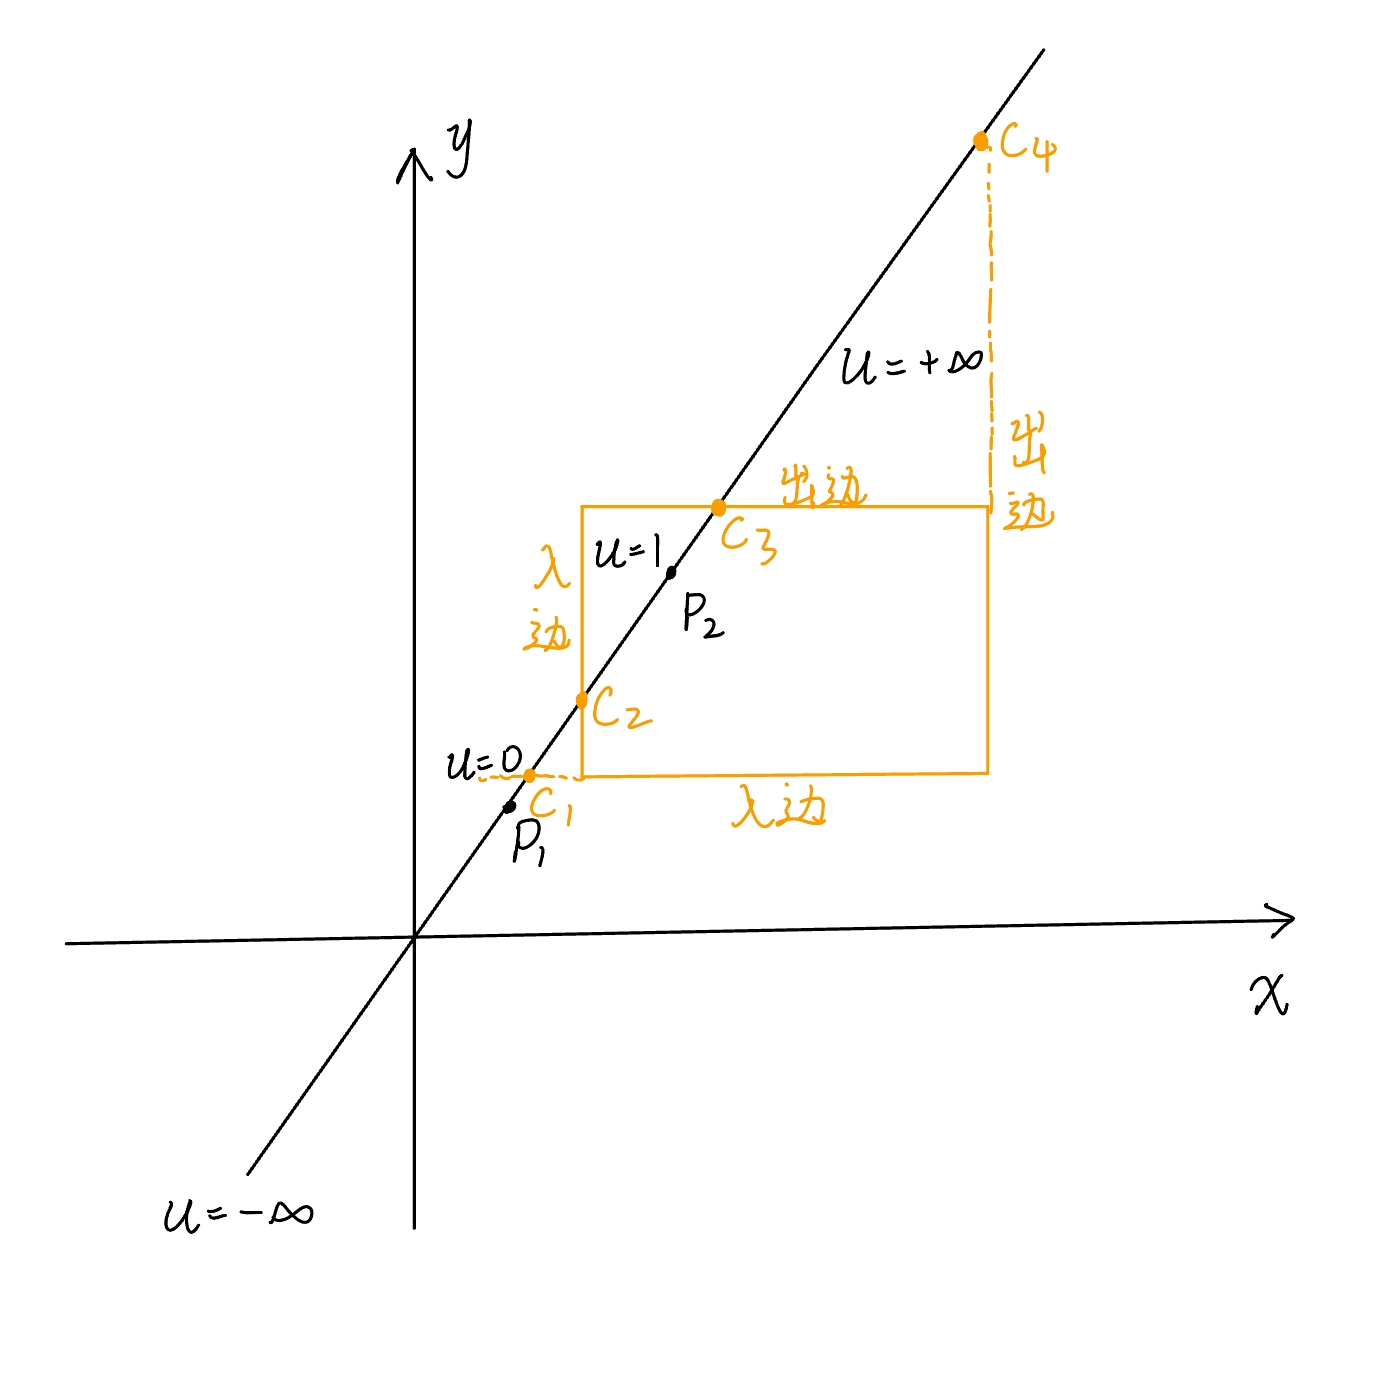
\includegraphics[width=4in]{报告/3.png}
\end{center}

显然裁剪得到的目标线段应该是$c_2$和$P_2$所夹线段,所以$u$的选取需要从$c_2$和$P_2$所对应的$u_1,u_2$入手,有以下关系:

$u_1=max(P_1,c_1,c_2)$,$u_1$是两个入边和$P_1$对应的$u$值的最大值;$u_2=min(P_2,c_3,c_4)$,$u_2$是两个出边和$P_2$对应$u$的最小值;且$u_1<u_2$。

因此问题转化为求出$c_1,c_2,c_3,c_4$所对应的$u$值,同时确定哪两条边是入边,哪两条边是出边。

对于第一个问题,结合上述等式组,考虑裁剪窗口的上边界为$y_{max}$,下边界为$y_{min}$,左边界为$x_{min}$,右边界为$x_{max}$,有:

\begin{center}
	$
	\begin{cases}  
		x_{min}\leq x_1 + u\Delta x\leq x_{max} \\
		y_{min}\leq y_1 + u\Delta y\leq y_{max}
	\end{cases} 
	$
\end{center}

于是当以下等式中某一条满足时,$u$所对应的值为裁剪直线和四个边界直线的交点。

\begin{center}
	$
	\begin{cases}  
		x_1 + u\Delta x = x_{min}	\\
		x_1 + u\Delta x = x_{max}	\\
		y_1 + y\Delta y = y_{min}	\\
		y_1 + u\Delta y = y_{max}
	\end{cases} 
	$
\end{center}

对于第二个问题,考虑上述不等式的一般情况:

\begin{center}
	$
	\begin{cases}  
		u(-\Delta x)\leq x_1 - x_{min}	\\
		u\Delta x\leq x_{max} - x_1	\\
		u(-\Delta y)\leq y_1-y_{min}	\\
		u\Delta y\leq y_{max} - y_1
	\end{cases} 
	$
\end{center}

可归纳为$up_k\leq q_k,k\in \{1,2,3,4\}$,当$p_k<0$时,线段从裁剪边界延长线的外部延伸到内部,即对应入边;当$p_k>0$时,线段从裁剪边界延长线的内部延伸到外部,即对应出边。同时当$p_k=0$时,若$q_k<0$,则线段完全在边界外;若$q_k>0$,则线段完全在边界内。

\subsubsection{算法实现}

需要实现或改动的函数有:

$\bullet$ start\_clip函数

$\bullet$ mousePressEvent函数

$\bullet$ mouseMoveEvent函数

$\bullet$ mouseReleaseEvent函数

$\bullet$ MainWindow类中连接槽函数,实现clip\_action函数

在start\_clip函数将当前系统状态调整为clip;在mousePressEvent函数中第一次点击确定裁剪窗口对角线的起始位置;在mouseMoveEvent函数中随着鼠标指针移动,实时更新裁剪窗口对角线另一端点的位置,然后调用alg.clip函数更新待裁剪线段的端点坐标,然后刷新界面。由此,即可实现裁剪功能。

\section{用户交互功能介绍}

\subsection{gui重置画布}

实现reset\_canvas\_action函数即可:

$\bullet$ 将所有画好的图形都删掉,并且将各参数重置为初始值

$\bullet$ 通过QDialog获取并记录新设置的宽和高

$\bullet$ 将画布的宽和高设置为Dialog中得到的宽和高

\subsection{gui保存画布}

添加save\_canvas\_act信号,实现save\_canvas\_action槽函数,并将其连接即可:

$\bullet$ 通过QFileDialog创建一个文件对话框对象,用于选择保存文件的路径和设置文件名

$\bullet$ 通过getSaveFileName获取并记录设置的文件名,并且限定文件类型为jpg、png和bmp格式

$\bullet$ 使用Pixmap对象,存储绘制的图像内容

\subsubsection{实现效果}

\begin{center}
	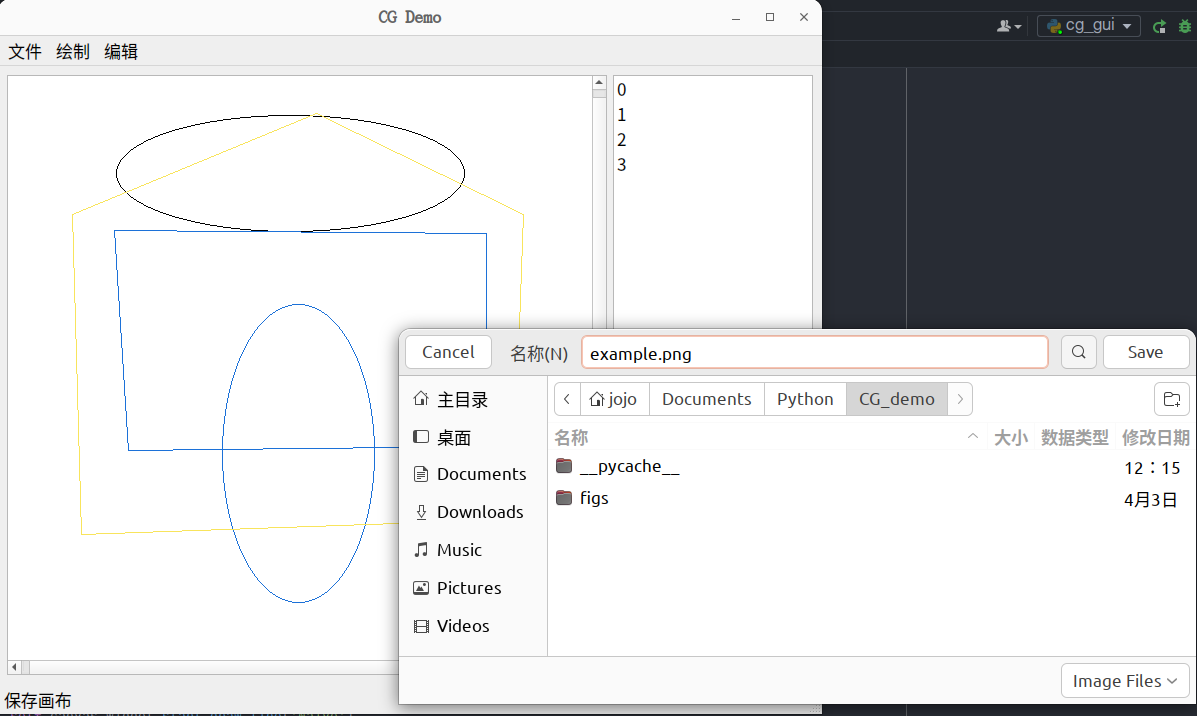
\includegraphics[width=6in]{报告/save.png}
	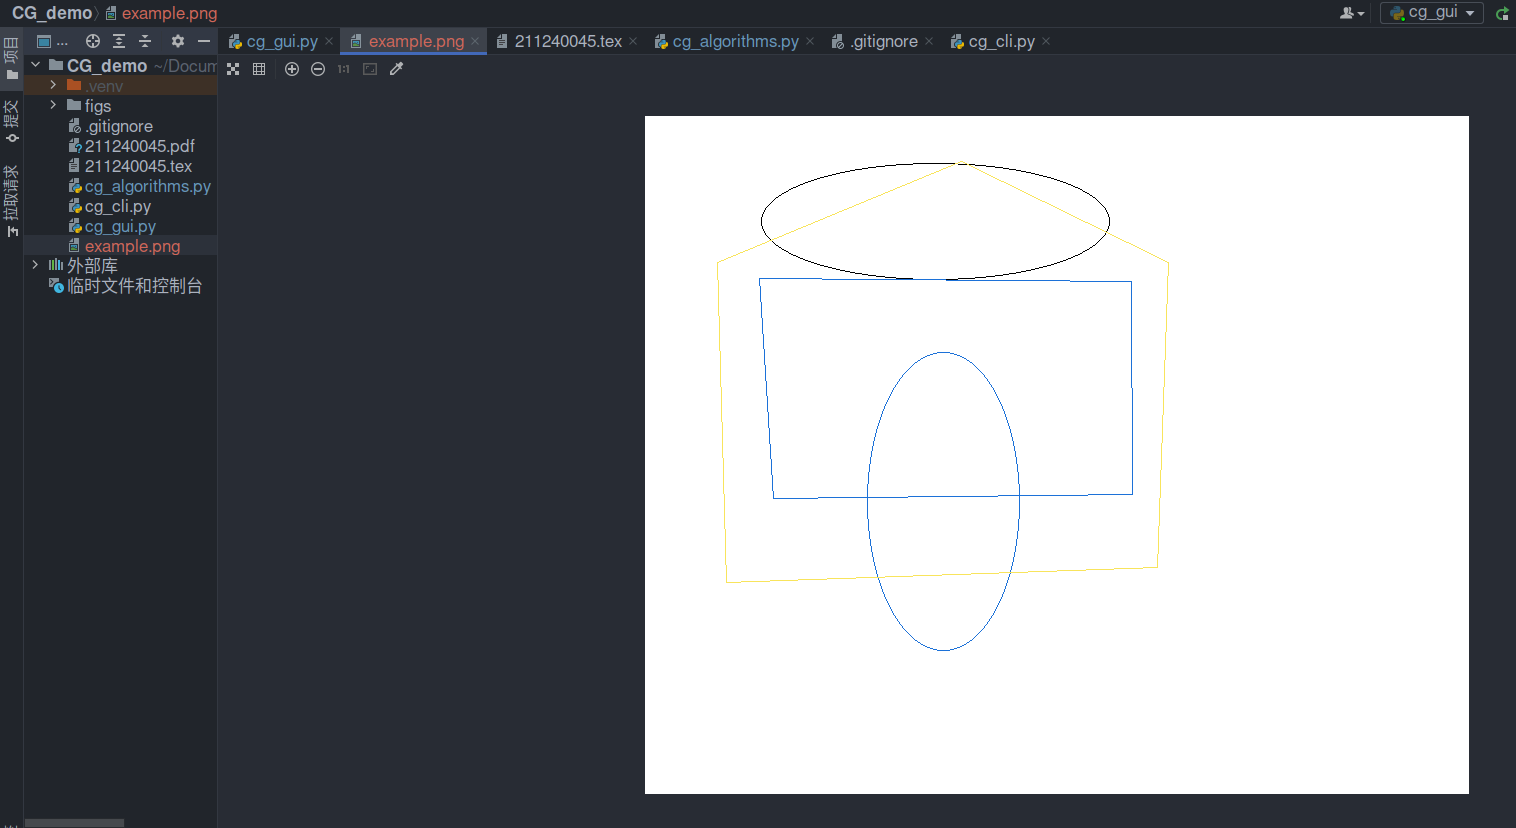
\includegraphics[width=6in]{报告/save_res.png}
\end{center}

\subsection{gui设置画笔颜色}

1. 首先实现set\_pen\_action函数:

$\bullet$调用QColorDialog类中的getColor函数获得新的颜色值

$\bullet$将颜色值存入画布的temp\_color成员中

2. 后在MyCanvas类中创建新的图形Item时,将temp\_color作为参数传入构造函数,初始化图形Item的color成员

3. 调用painter.drawPoint函数画图前,使用setPen函数设置画笔颜色,保证图形颜色符合预期

\subsubsection{实现效果}

\begin{center}
	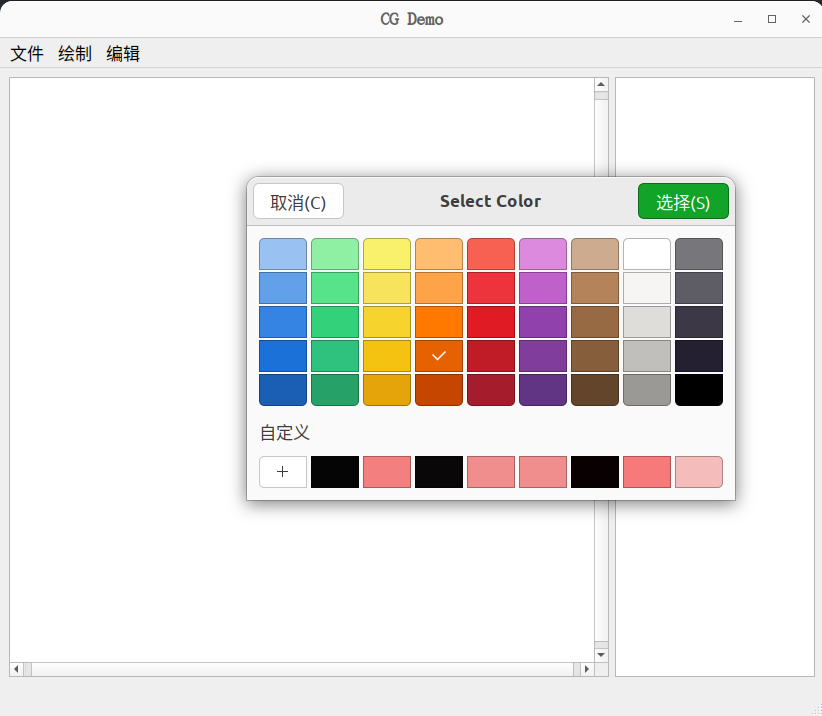
\includegraphics[width=6in]{报告/color1.png}
	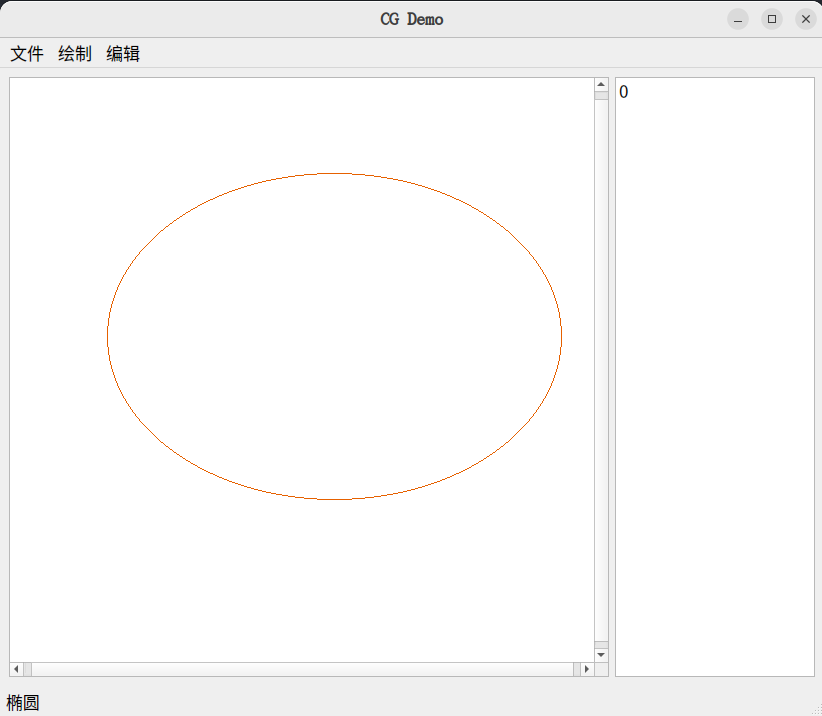
\includegraphics[width=6in]{报告/color2.png}
\end{center}

\subsection{cli命令行界面}

使用readline()方法读取指令文件中的命令,使用line.strip().split(' ')拆分传入的参数。对于绘图指令,需要将传入的关键参数保存;对于图元变换指令,需要调用算法库(cg\_algorithms.py)中的对应图元变换函数生成新的点坐标集(pointSet),并存入item\_dict;对于保存指令,需要根据图元类型调用算法库(cg\_algorithms.py)中的对应图元绘制函数生成待绘制点集(pixels),然后保存为.bmp文件。

值得注意的是,在实验手册中规定绘制坐标系的坐标原点在屏幕左上方(往右为x正方向,往下为y正方向),因此将模板程序中的canvas[height - 1 - y, x]修改为canvas[y, x]。

\section{总结}
本次《计算机图形学》课程实验历时三个月,在这段时间我使用python语言实现了课程中讲授的各种图形学算法,并结合PyQt5库,最终完成了一个具有图形界面的完整的图形学系统。

在完成课程实验的过程中,我加深了对DDA、Bresenham、Cohen-Sutherland、Liang-Barsky等图形绘制算法的理解,同时对《计算机图形学》这门课程的应用场景有了更加深刻的认识。当然这个过程不是一帆风顺的,我在将图形学的理论(公式)用python代码实现时经常会遇到一些奇怪的bug,比如浮点数整数未转换、除0错等。上述问题经过不断调试和优化代码都得到了解决,并且我逐渐掌握了解决图形学程序中疑难问题的能力,同时我的代码工程能力也得到了增强。

通过这这次大作业,我不仅加深了对计算机图形学基础知识的理解,还提升了自己的编程技能和创造力。这段经历让我更加热爱图形学领域,同时也为将来的学习和工作打下了坚实的基础。
\end{document}